\documentclass[a4paper,12pt]{article}

%%% Работа с русским языком
\usepackage{cmap}					% поиск в PDF
\usepackage{mathtext} 				% русские буквы в фомулах
\usepackage[T2A]{fontenc}			% кодировка
\usepackage[utf8]{inputenc}			% кодировка исходного текста
\usepackage[english,russian]{babel}	% локализация и переносы

%\usepackage{biblatex} %Imports biblatex package

\usepackage{subcaption}
\usepackage{graphicx}
\usepackage{makecell}
\usepackage{hyperref}

%%% Дополнительная работа с математикой
\usepackage{amsfonts,amssymb,amsthm,mathtools} % AMS
\usepackage{amsmath}
\usepackage{icomma} % "Умная" запятая: $0,2$ --- число, $0, 2$ --- перечисление
\usepackage{amsthm}

%% Номера формул
%\mathtoolsset{showonlyrefs=true} % Показывать номера только у тех формул, на которые есть \eqref{} в тексте.

%% Шрифты
\usepackage{euscript}	 % Шрифт Евклид
\usepackage{mathrsfs} % Красивый матшрифт

%% Свои команды
\DeclareMathOperator{\sgn}{\mathop{sgn}}

%% Перенос знаков в формулах (по Львовскому)
\newcommand*{\hm}[1]{#1\nobreak\discretionary{}
	{\hbox{$\mathsurround=0pt #1$}}{}}

%%% Работа с картинками
\usepackage{graphicx}  % Для вставки рисунков
\graphicspath{{images/}{images2/}}  % папки с картинками
\setlength\fboxsep{3pt} % Отступ рамки \fbox{} от рисунка
\setlength\fboxrule{1pt} % Толщина линий рамки \fbox{}
\usepackage{wrapfig} % Обтекание рисунков и таблиц текстом
\usepackage{caption}
\captionsetup{labelsep=period} %. вместо : в рис

%%% Работа с таблицами
\usepackage{array,tabularx,tabulary,booktabs} % Дополнительная работа с таблицами
\usepackage{longtable}  % Длинные таблицы
\usepackage{multirow} % Слияние строк в таблице

\usepackage{extsizes} % Возможность сделать 14-й шрифт
\usepackage{geometry} % Простой способ задавать поля
\geometry{top=25mm}
\geometry{bottom=35mm}
\geometry{left=10mm}
\geometry{right=15mm}

\begin{document}
	
	\begin{titlepage}
		\begin{center}
			
			\vspace{0.5cm}
			\large
			Московский физико-технический институт 
			
			(национальный исследовательский университет)
			\vspace{0.25cm}
			
			Физтех-школа радиотехники и компьютерных технологий \\
			
			Кафедра мультимедийных технологий и телекоммуникаций
			\vfill
			
			\textsc{Практическое задание №1}\\[5mm]
			
			{\LARGE Энтропия языка}
			\bigskip
			
			Назмиев Айрат, 5 курс, группа М01-305
		\end{center}
		\vfill
		
		\newlength{\ML}
		\settowidth{\ML}{«\underline{\hspace{0.7cm}}» \underline{\hspace{2cm}}}
		
		\vfill
		\vfill
		
		\begin{center}
			Москва, 2024 г.
		\end{center}
		
	\end{titlepage}
	
	\section*{Цель работы}
	В данной работе требуется провести оценку энтропии текста на естественном языке. Оценка производится при помощи последовательных оценок n-граммных условных энтропий $F_n$ и n-мерной средней энтропии на букву $H_n$. Также находится средняя энтропия слова на букву. Для анализы выбраны несколько художественных текстов на русском и английском языках.
	
	\section*{Введение}
	Энтропия есть статистический параметр, который измеряет в известном
	смысле среднее количество информации, приходящейся на одну букву языкового текста. Если данный язык перевести на язык двоичных знаков (0 или 1) наиболее эффективным образом, то двоичная энтропия $H$ равна среднему числу
	двоичных знаков (бит), приходящихся на одну букву исходного языка \cite{fominykh2024}. Энтропия дискретного ансамбля $X = \{x,\,p(x)\}$ определяется следующим образом:
	
	\begin{equation}\label{key}
		H(X) = 
		\mathbb{E}\left[-\log p(x)\right] = 
		- \sum\limits_{x\in X} p(x) \log p(x).
	\end{equation}

	В нашем случае $X$ является символами текста, а точнее буквы алфавита и символ пробела. Здесь и всюду ниже логарифм берется по основанию 2, единицей измерения является бит. Можно заметить, что $ H(X) \ge 0 $ (из $ p(x) \in [0;\; 1] $) и $ H(X) \le \log_2 |X|$ (максимум энтропии достигается при равномерном распределении символов).
	
	Введем понятие условной энтропии. Рассмотрим второй дискретный ансамбль $Y = \{y,\,p(y)\}$, произведением ансамблей является $ XY = \{(x,\,y),\,p(x,\,y)\} $. Условная энтропия $X$ при условии $Y$ определяется как:
	
	\begin{equation}\label{key}
		H(X|Y) = 
		\mathbb{E}_Y\left[ -\sum\limits_{x\in X} p(x|y) \log p(x|y) \right] = 
		- \sum\limits_{x\in X} \sum\limits_{y\in Y} p(x,\,y) \log p(x|y).
	\end{equation}

	Из определения следует, что $ H(X|Y) \ge 0 $. Кроме того, добавление условия не увеличивает энтропию, то есть $ H(X|Y) \le H(X) $, равенство достигается только при независимости $ X $ и $Y$. Из цепного правила для вероятностей можно вывести цепное свойство энтропии:
	
	\begin{equation}\label{eq:Hchain}
		H(X_1...X_n) = H(X_1) + H(X_2 | X_1) + ... + H(X_n|X_1...X_{n-1}).
	\end{equation}

	Как можно видеть, при добавлении случайной величины энтропия не уменьшается. Текст рассматривается нами как стационарный источник, поэтому можно ввести понятие n-мерной энтропии текста: $ H(X_1...X_n) = H(X^n) $, то есть здесь нет зависимости от позиции блока букв в тексте. $ H(X^n) $, нормированная на блока $ n $, называется n-мерной средней энтропией на букву:  
	
	\begin{equation}\label{key}
		H_n(X) = \frac{H(X^n)}{n}.
	\end{equation}
	
	При увеличении $ n $ величина $ H_n(X) $ может являться оценкой энтропии стационарного источника $ H $. Другим подходом к оценке $ H $ явлется рассмотрение условных n-граммных энтропий:
	
	\begin{equation}\label{key}
		F_n = H(X_n|X_1...X_{n-1}) = H(X|X^{n-1}).
	\end{equation}

	Из-за стационарности источника индексы также могут быть опущены. Заметим, что из определения $ F_n $ и \ref{eq:Hchain} следует, что $ F_n = H(X^n) - H(X^{n-1})$. 
	
	Опишем основные свойства $ H_n(X) $ и $ F_n(X) $.  $ F_n(X) $ и $H_n(X)$ не возрастают при росте $ n $. Для $ F_n(X) $ это сразу следует из невозрастания энтропии при добавлении условия, а для доказательства утверждения с $H_n(X)$ предварительно также нужно использовать свойство \ref{eq:Hchain} и неотрицательность энтропии. Из свойства \ref{eq:Hchain} также следует неравенство $H_n(X) \ge F_n(X) $.
	Энтропия стационарного источника вводится как предел при стремлении размера блока/глубины памяти к бесконечности, при этом пределы для $H_n(X)$ и $ F_n(X) $ совпадают:
	
	\begin{equation}\label{eq:H_inf}
		H = \lim\limits_{n\rightarrow \infty} H_n(X) = \lim\limits_{n\rightarrow \infty} F_n(X).
	\end{equation}

	Из-за ограниченности вычислительных ресурсов и данных, в работе для оценки $ H $ будут рассмотрены $ N $ до 6 включительно.
	
	\section*{Эксперимент}
	
	Рассмотрим по три текста на русском и английском языках: <<Мастер и Маргарита>> Булгакова, <<Доктор Живаго>> Пастернака, <<The Tragedy of Hamlet, Prince of Denmark>> Шекспира, <<1984>> Оруэлла. В работе также используется <<Война и Мир>> Толстого на двух языках, также рассмотрен вариант объединения трех текстов для каждого из языков в один. Построим зависимости последовательных приближений $F_n$, $n=\overline{0,\,6}$. Также найдем энтропию по словам и посчитаем для нее среднюю энтропию на букву. Пробел считаем символом, разбиение текста на блоки происходит с перекрытием. Результаты приведены в таблице \ref{table:Fn}.
	
	\begin{table}[h!]
		\centering
	\begin{tabular}{|c|c|c|c|c|c|c|c|c|c|c|c|c|}
		\hline
		& Text & \#Symbols & Alphabet & $F_0$ & $F_1 $ & $F_2$ & $F_3$ & $F_4$ & $F_5$ & $F_6$ & $F_{\text{word}}$ \\
		\hline
		1 & <<1984>> & 569310 & 27 & 4.76 & 4.09 &  3.30 & 2.65 & 2.05 & 1.64 & 1.33 & 2.15 \\
		\hline
		2 & <<Hamlet>> & 163012 & 27 & 4.76 & 4.07 & 3.31 & 2.63 & 2.05 & 1.62 & 1.22 &  2.34 \\
		\hline
		3 &<<War \& Peace>> & 3107847 & 27 & 4.76 &  4.08 & 3.31 & 2.67 & 2.09 & 1.73 & 1.49 & 2.24 \\
		\hline
		4 & 1-3 & 3840171 & 27 & 4.76 & 4.08 & 3.32 & 2.69 & 2.13 & 1.77 &  1.54 & 2.24 \\
		\hline
		5 & <<Мастер и Маргарита>> & 712333 & 33 & 5.04 & 4.37 & 3.59 & 3.01 & 2.35 & 1.82 & 1.36 & 2.18\\
		\hline
		6 & <<Доктор Живаго>> & 1007311 & 34 & 5.09 & 4.4 & 3.59 & 3.03 & 2.47 & 1.97 & 1.52 & 2.25\\
		\hline
		7 & <<Война и Мир>> & 2750968 & 34 & 5.09 & 4.38 & 3.56 & 2.92 & 2.31 & 1.89 & 1.58 & 2.22 \\
		\hline
		8 & 5-7 & 4470614 & 34 & 5.09 & 4.38 & 3.58 & 3.00 & 2.42 & 2.01 &  1.7 & 2.29\\
		\hline
	\end{tabular}
	\caption{Приближения $F_n$}
	\label{table:Fn}
	\end{table}

	Можно видеть, что $F_n$ при росте длины контекста не возрастает. Самую длинную из рассмотренных ($ n=6 $) условных энтропий можем рассматривать как грубую оценку энтропии источника (языка). Из-за ограниченности выборки текстов дальнейшее увеличение $ n $ не приводит к сходимости истинной энтропии $ H $, $F_n$ стремится к нулю, так как достаточно длинный контекст для данной выборки будет уникален и с вероятностью 1 определять дальнейший символ. Кроме приближений $F_n$ также были найдены $ H_n $, но чтобы не загромождать таблицу, они не были приведены в отчете. Также рассмотрение групп символов без перекрытия снижает выборку, что приводит к заниженным оценкам $F_n$ и  $H_n$. Средние длины слов на английском и русском оказались равны 4.30 и 5.21 соответственно. Даже с учетом довольно ограниченной выборки, оценка $ F_n $ и энтропия на букву в словах оказались довольно близки для соответствующих длин слов ($ n=3-4$ для английского и $ n=4-5$ для русского языка). Однако важны также и взаимосвязи между словами, фразами, более длинные статистические связи, которые принципиально не могут быть учтены в $F_{\text{word}}$. Также длины слов могут изменяться в широких диапазонах от одной буквы (предлоги, артикли) до нескольких десятков, что дополнительно ограничивает уместность сравнения. Кроме того, при подсчете $F_n$ используется пробел. В <<Мастер и Маргарита>> 33 символа, так как в тексте не используется буква <<ё>>.

	
	В качестве примера ниже будет дан график для $F_n$ и $ H_n $ объединенного текста соответственно на английском и русском языках (рис. \ref{fig:sym_word}).
	
	\begin{figure}[h!]
		\centering
		\begin{subfigure}{0.3\linewidth}
			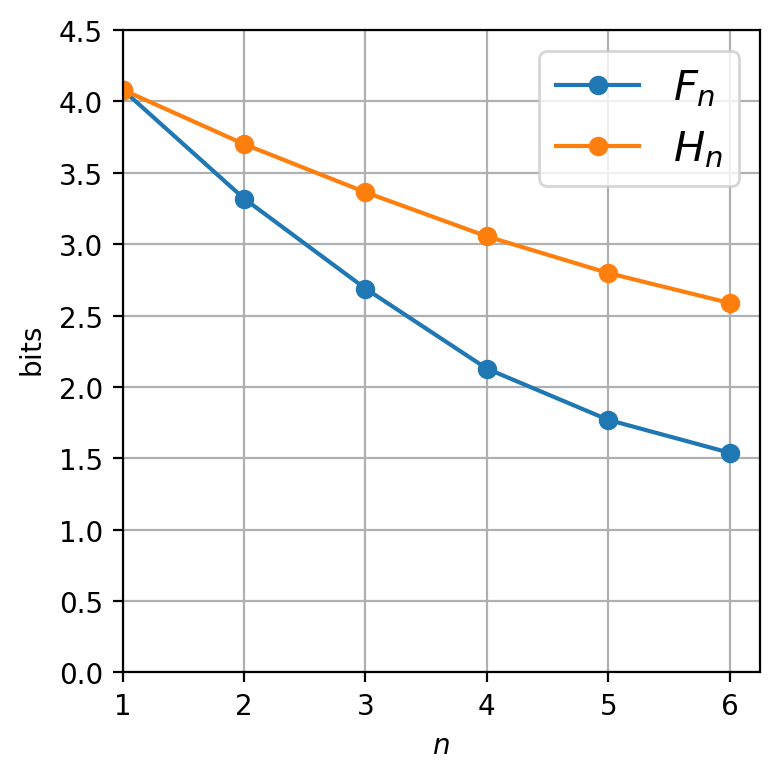
\includegraphics[width=\linewidth]{figs/F_H_en}
			\caption{Текст на английском}
			\label{fig:F_H_en}
		\end{subfigure}
		\begin{subfigure}{0.3\linewidth}
			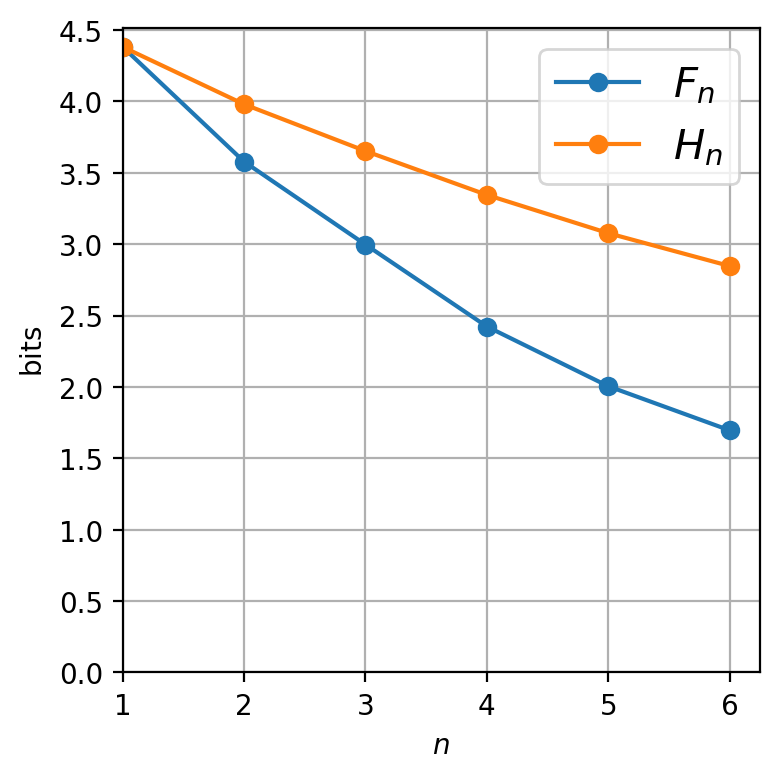
\includegraphics[width=\linewidth]{figs/F_H_ru}
			\caption{Текст на русском}
			\label{fig:F_H_ru}
		\end{subfigure}
		\caption{Энтропии $F_n$ и $H_n$}
		\label{fig:F_H}
	\end{figure}

	На графиках можно увидеть, что $F_n$ и $ H_n $ являются невозрастающими функциями от $ n $, кроме того, выполняется $H_n(X) \ge F_n(X) $, что согласуется с теоретическими результатами. Текст на русском оказывается заметно более избыточным, чем на английском, что особенно видно при сравнении переводного текста (на примере романа <<Война и Мир>>). Построим гистограммы символов и наиболее частых слов для обоих языков:
	
	\begin{figure}[h!]
		\centering
		\begin{subfigure}{0.48\linewidth}
			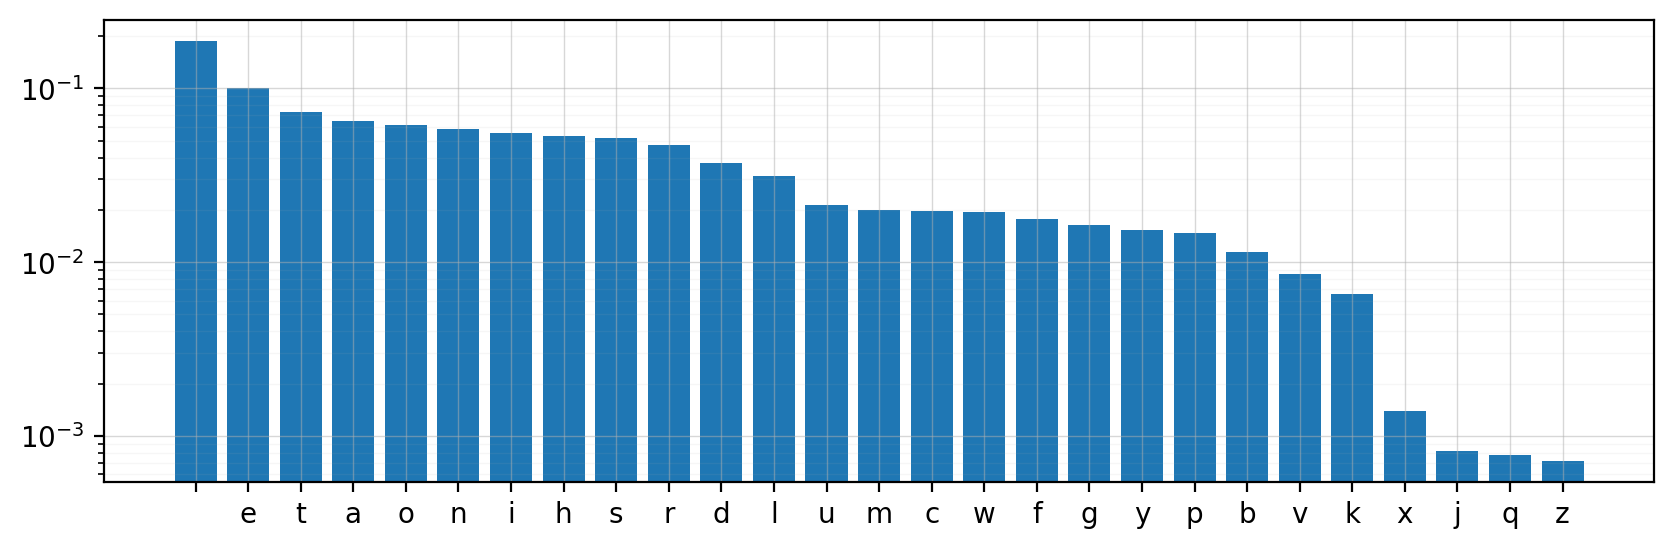
\includegraphics[width=\linewidth]{figs/sym_en}
		\end{subfigure}
		\begin{subfigure}{0.48\linewidth}
			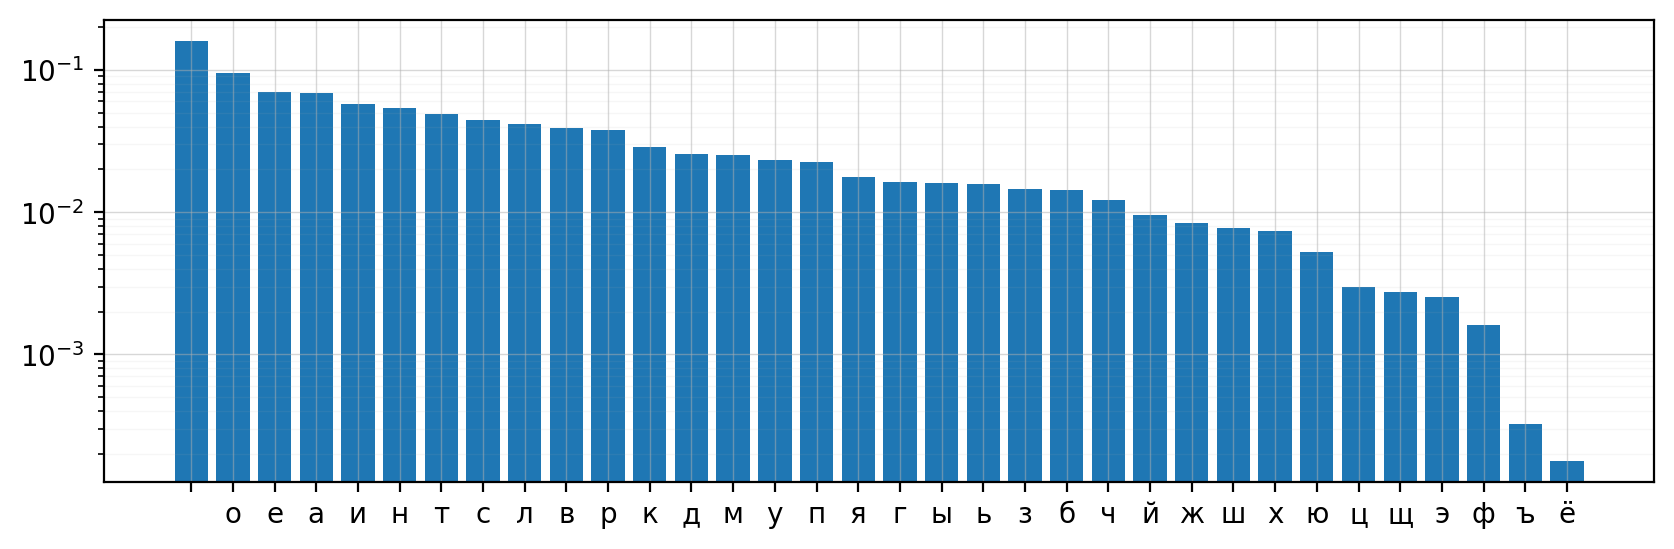
\includegraphics[width=\linewidth]{figs/sym_ru}
		\end{subfigure}
		\\
		\begin{subfigure}{0.48\linewidth}
			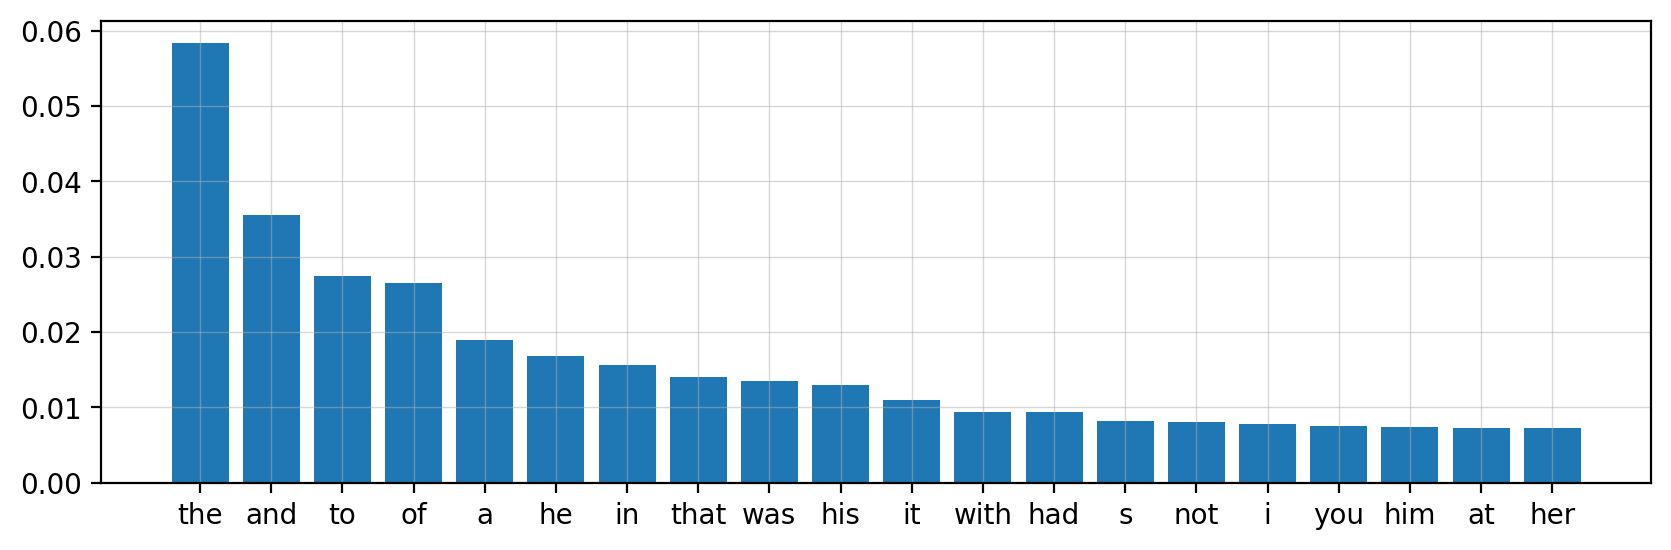
\includegraphics[width=\linewidth]{figs/word_en}
		\end{subfigure}
		\begin{subfigure}{0.48\linewidth}
			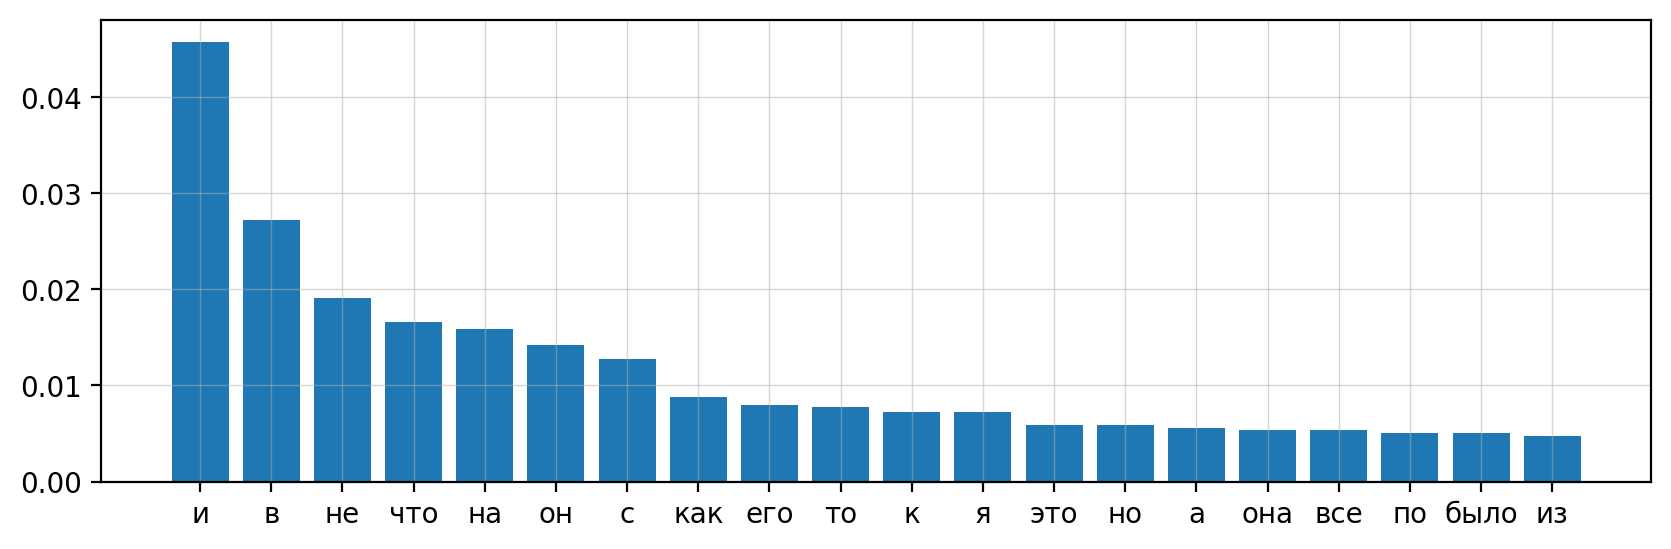
\includegraphics[width=\linewidth]{figs/word_ru}
		\end{subfigure}
		\caption{Частоты букв (символов) и наиболее распространенных слов}
		\label{fig:sym_word}
	\end{figure}

	Ожидаемо, для английского самыми распространенными словами являются артикли и предлоги, а для русского "--- предлоги и частицы. В обоих языках чаще всего встречается пробел, а в русском самыми частотными, очевидно, являются несколько гласных.
	
	\section*{Выводы}
	
	В ходе работы были произведены оценки n-граммных условных энтропий $F_n$ и n-мерных средних энтропии на букву $H_n$, данные подтверждают основные свойства условной и многомерной энтропии. Шеннон оценил энтропию английского языка в 1.3 бит/символ \cite{shannon1951H}, полученная величина условной энтропии $ F_6 = 1.54 $ бит/символ оказалась довольно близка к шенноновской, но, однако, по построению не учитывает длинные зависимости в тексте.
	
	
	\clearpage
	\newpage
	\begin{thebibliography}{0}
		\addcontentsline{toc}{section}{\refname}
		\bibitem{shannon1948comm} Shannon, C. E. A Mathematical Theory of Communication, 1948
		
		\addcontentsline{toc}{section}{\refname}
		\bibitem{shannon1951H} Shannon, C. E. Prediction and Entropy of Printed English, 1951
		
		\addcontentsline{toc}{section}{\refname}
		\bibitem{fominykh2024} Фоминых, А. Лекции по курсу <<Семантическое кодирование>>, 2024
		
		%\addcontentsline{toc}{section}{\refname}
		%\bibitem{matlab2023cfar} The Math Works, Inc. \href{https://www.mathworks.com/help/radar/ug/cfar-detection.html?searchHighlight=cfar\&s\_tid=srchtitle\_support\_results\_2\_cfar}{Constant False Alarm Rate (CFAR) Detection.}
		
		
		
	\end{thebibliography}
	
	
\end{document}